% Figure: how the pieces of the proof fit together
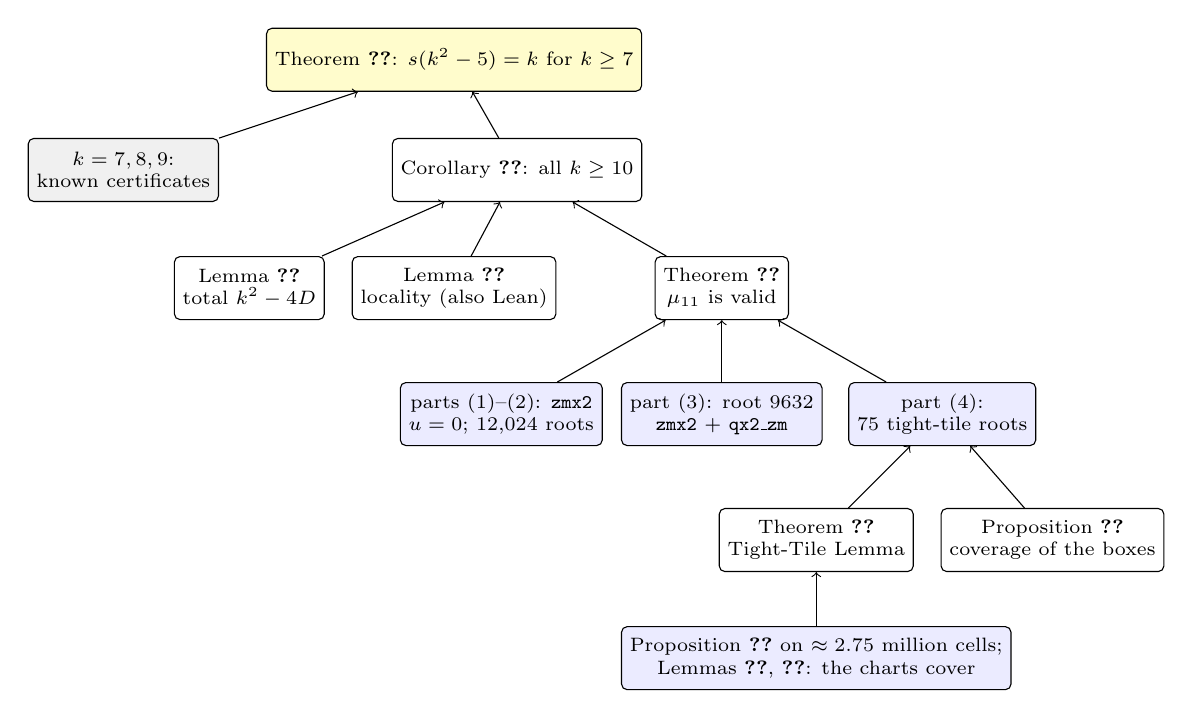
\begin{tikzpicture}[font=\scriptsize,
  box/.style={draw,rounded corners=2pt,align=center,inner sep=3pt,fill=white,minimum height=0.8cm},
  comp/.style={box,fill=blue!8}, ext/.style={box,fill=gray!12}]
  \node[box,fill=yellow!20] (main) at (0,0) {Theorem~\ref{thm:main}: $s(k^2-5)=k$ for $k\ge7$};
  \node[ext] (base) at (-4.2,-1.4) {$k=7,8,9$:\\ known certificates};
  \node[box] (cor) at (0.8,-1.4) {Corollary~\ref{cor:reduce}: all $k\ge10$};
  \node[box] (mass) at (-2.6,-2.9) {Lemma~\ref{lem:mass}\\ total $k^2-4D$};
  \node[box] (loc) at (0,-2.9) {Lemma~\ref{lem:local}\\ locality (also Lean)};
  \node[box] (valid) at (3.4,-2.9) {Theorem~\ref{thm:valid}\\ $\mu_{11}$ is valid};
  \node[comp] (p1) at (0.6,-4.5) {parts (1)--(2): \texttt{zmx2}\\ $u=0$; $12{,}024$ roots};
  \node[comp] (p3) at (3.4,-4.5) {part (3): root $9632$\\ \texttt{zmx2} + \texttt{qx2\_zm}};
  \node[comp] (p4) at (6.2,-4.5) {part (4):\\ $75$ tight-tile roots};
  \node[box] (tt) at (4.6,-6.1) {Theorem~\ref{thm:tt}\\ Tight-Tile Lemma};
  \node[box] (cov) at (7.6,-6.1) {Proposition~\ref{prop:coverage}\\ coverage of the boxes};
  \node[comp] (cells) at (4.6,-7.6) {Proposition~\ref{prop:cell} on $\approx2.75$ million cells;\\ Lemmas~\ref{lem:charts}, \ref{lem:corners}: the charts cover};
  \draw[->] (base) -- (main); \draw[->] (cor) -- (main);
  \draw[->] (mass) -- (cor); \draw[->] (loc) -- (cor); \draw[->] (valid) -- (cor);
  \draw[->] (p1) -- (valid); \draw[->] (p3) -- (valid); \draw[->] (p4) -- (valid);
  \draw[->] (tt) -- (p4); \draw[->] (cov) -- (p4); \draw[->] (cells) -- (tt);
\end{tikzpicture}
